\documentclass[11pt]{beamer}
\usepackage[UTF8]{ctex}
\usepackage[utf8]{inputenc}
\usepackage[T1]{fontenc}
\usepackage{lmodern}
\usepackage{amsmath}
\usepackage{amsfonts}
\usepackage{amssymb}
\usepackage{graphicx}
\usetheme{CambridgeUS}

\usepackage{pdfpages}


%%%%%
\usepackage{longtable}
\usepackage{subfigure}
\usepackage{color}
\usepackage{booktabs}

%%%%%
\usepackage[backend=bibtex,sorting=none]{biblatex}
\addbibresource{reference.bib} %BibTeX数据文件及位置
\setbeamerfont{footnote}{size=\tiny} 
\setbeamertemplate{bibliography item}[text]

%% LOGO放右上
\setbeamertemplate{frametitle}
{\begin{beamercolorbox}[wd=\paperwidth]{frametitle}
		\strut\hspace{0.5em}\insertframetitle\strut
		\hfill
		\raisebox{-2mm}{
\includegraphics[width=1cm]{figures/HNUC.jpeg}}
	\end{beamercolorbox}
}

\begin{document}
\author{郭泰彪}
\title{区块链原理及应用}
\subtitle{第3课:区块链的信任基础}
\begin{frame}[plain]
\institute{湖南工商大学大数据与互联网创新研究院}
\date{2020年9月24日}

	\maketitle
\end{frame}

\begin{frame}
	\frametitle{目录}
	\tableofcontents[sectionstyle=show,subsectionstyle=show/shaded]
\end{frame}

\section{导言:生活中的信任}

\subsection{社会现象背后的信任断层}

\subsection{中国传统的血缘信任}

\subsection{中国传统的血缘信任}

\subsection{西方现代社会的制度化信任}
\begin{frame}{信任的定义}

\end{frame}

\section{两种典型的信任模式}

\subsection{基于记忆的信任模式}

\subsection{通过可信第三方的信任模式}

\section{陌生人间建立信任的问题}

\section{问题推广:不可信机器间建立信任的问题}
\begin{frame}{问题推广:不可信机器间建立信任的问题}
	一个可靠的计算机系统必须能够应付一个或多个组件发生故障。一个失败的组件可能会表现出一种经常被忽视的行为,向系统的不同部分发送冲突的信息。
\end{frame}

\begin{frame}{几个名词的辨析的区别}
	分布式系统的故障:进程或通信通道偏离被认为是正确或期望的行为。
	\begin{enumerate}
		\item 进程故障: 
		\item 通信故障:
		\end{enumerate}
	
	\begin{enumerate}
		\item 进程故障: 
		\item 通信故障:
	\end{enumerate}
\end{frame}

\begin{frame}{利用分布式系统来解决可靠性的例子}
	\begin{figure}
		\centering
		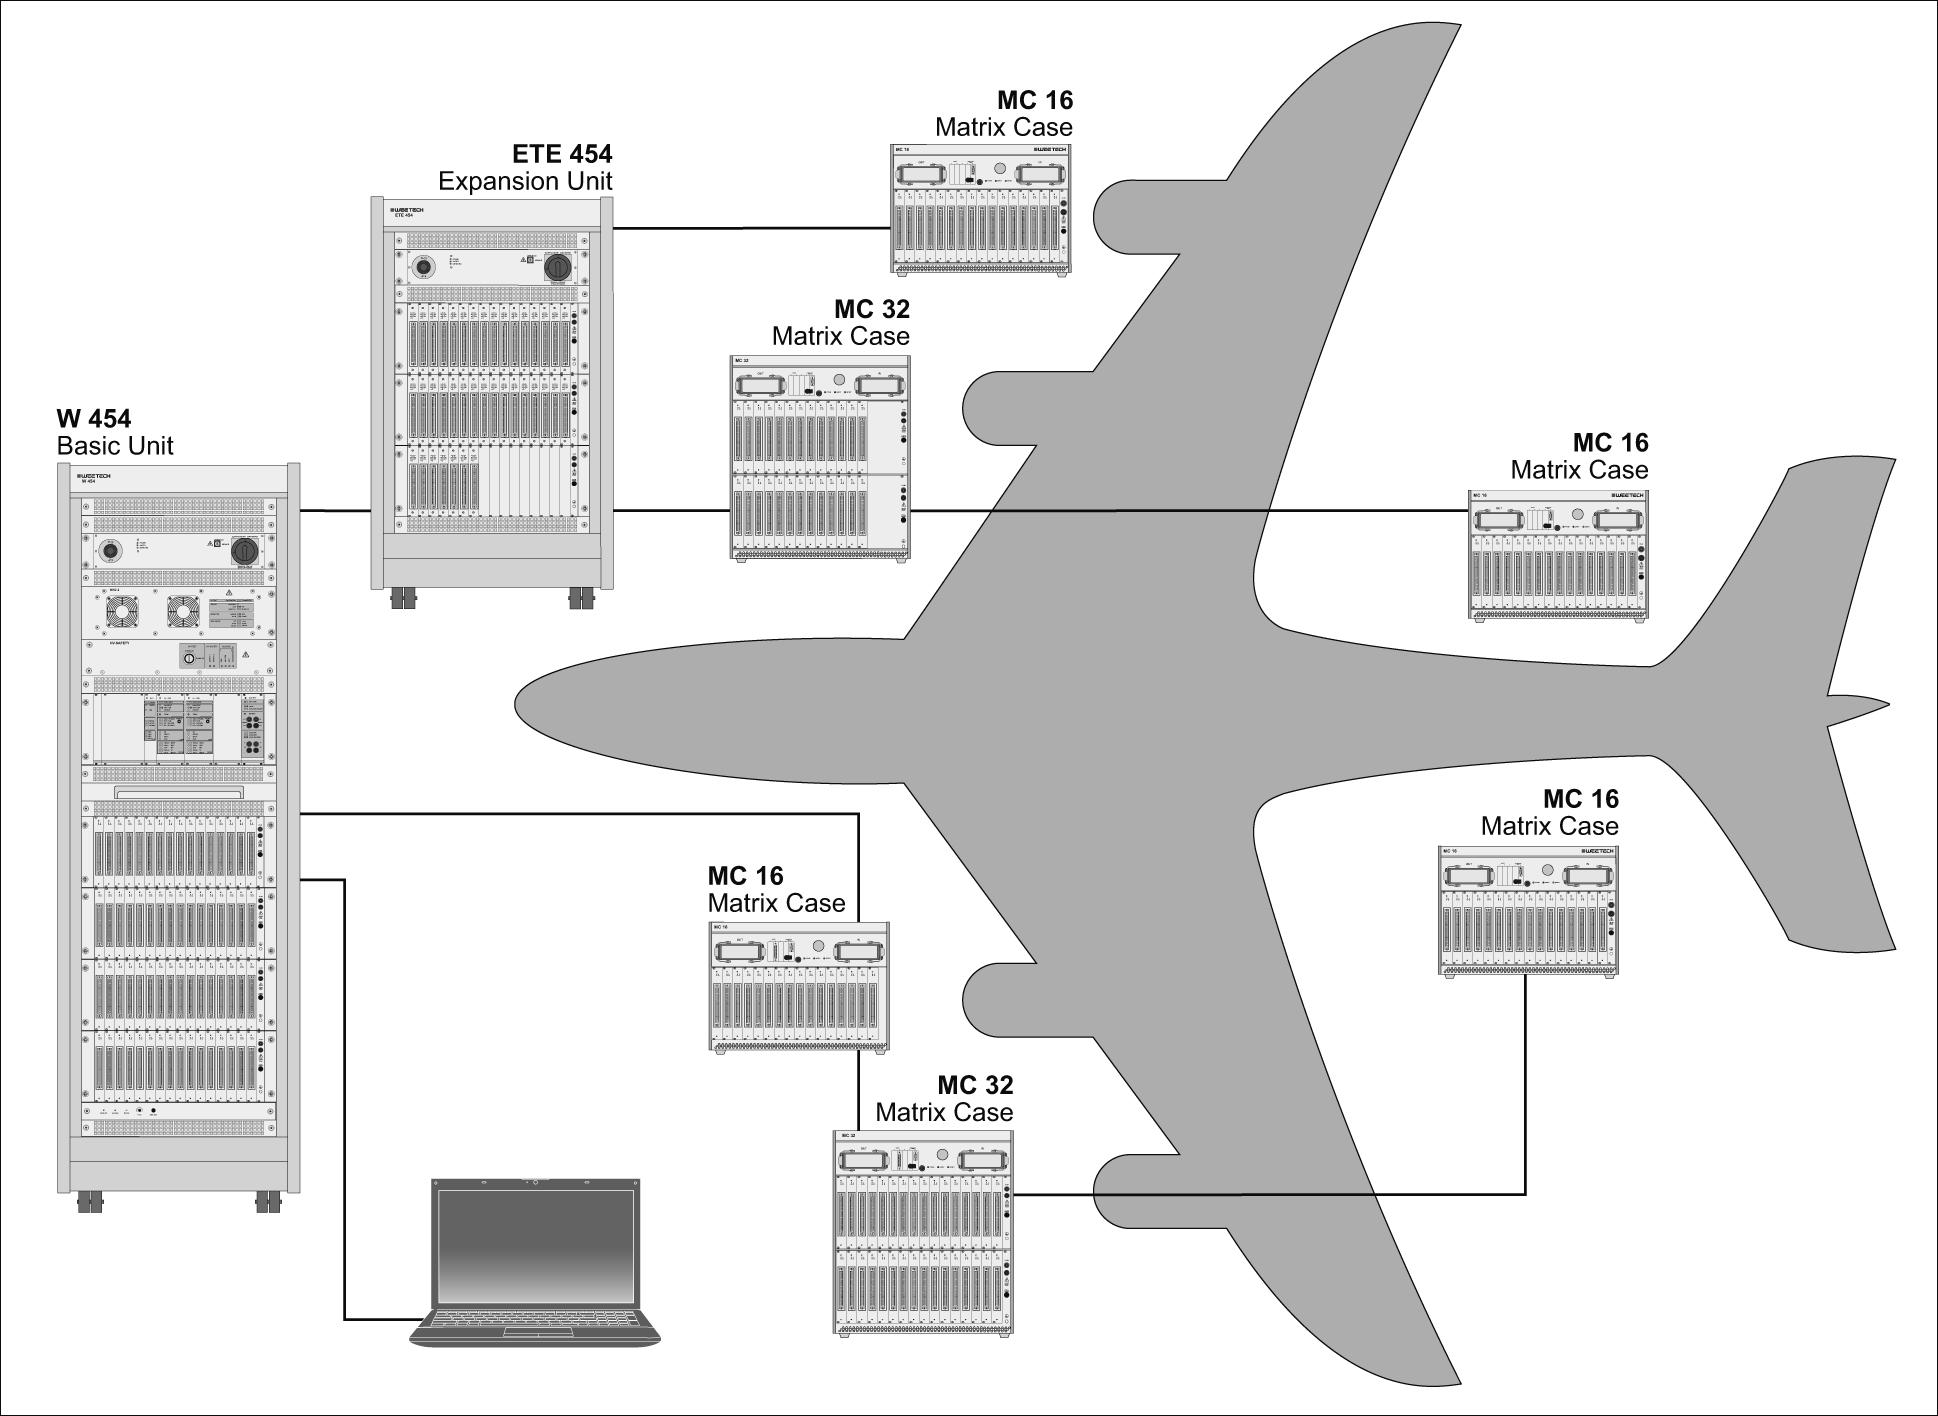
\includegraphics[width=0.7\linewidth]{figures/distributedPlane}
		\caption{飞机利用分布式系统来确保机载计算机系统可靠性}
		\label{fig:distributedplane}
	\end{figure}
	
\end{frame}

% 在网络中存在恶意者的情况下完成程序的执行
\section{问题的抽象化:拜占庭将军问题}

\begin{frame}{拜占庭将军问题背景}
	处理这类失败的问题被抽象地表述为拜占庭将军问题\cite{lamport_byzantine_1982}。
	\begin{enumerate}
		\item 角色定义:COMMANDER()、LIEUTENANT
		\item 
	\end{enumerate}
\end{frame}

\section{区块链:“虚拟”可信第三方}

\section{区块链如何解决陌生人信任问题}

\section{问题分解}

\section{参考文献}
\begin{frame}{参考文献}
	\printbibliography
\end{frame}

\section*{谢谢聆听}

\begin{frame}
	\begin{minipage}[t]{0.5\linewidth}
		\begin{center}
			\begin{figure}
				\vspace{10pt}
				
				{\Huge 谢谢聆听}
				
				\vspace{30pt}
				郭泰彪
				
				\vspace{10pt}
				{\tiny 湖南工商大学大数据与互联网创新研究院}
			\end{figure}
			\begin{figure}
				
			\end{figure}
		\end{center}
	\end{minipage}%
	\begin{minipage}[t]{0.4\linewidth}
		\begin{figure}
			\centering
			\texttt{blockchain101}
			
			
\includegraphics[width=0.6\linewidth]{figures/blockchain101qrcode}
			
			{\footnotesize \texttt{Star| Fork| Issue}}
		\end{figure}
	\end{minipage}%
\end{frame}

\end{document}